\documentclass{article}

\usepackage{tikz}
\usepackage{pgfplots}
\usepackage{verbatim}

\usepackage[top=1in, bottom=1.5in, left=1in, right=1in]{geometry}

\usepackage{graphicx}

\author{Stefan Seritan (PERM: 5466644), Wei Dai (CSIL: wdai, PERM: 6925747)}
\date{\today}
\title{CS140 Final Project Proposal:\\A Parallel Metropolis Monte Carlo Simulation}

\begin{document}
\maketitle

\section*{Background}
\vspace{-7pt}
\indent\indent Simulations are a powerful tool to test and explore different chemical and physical models. In chemistry, two main types of simulations are utilized: Molecular Dynamics (MD) and Monte Carlo (MC). In MD simulations, an initial state is propagated through time to a final state using classical physics. The galactic evolution project (Homework 3) was an example of an MD-type simulation. Unlike MD simulations, Monte Carlo simulations are governed by statistical mechanics, not classical mechanics. As a result, MC simulations can perform unphysical moves, reaching equilibrium quickly (but losing any dynamic information). The principle of ergodicity states that the results of an MD and MC simulation will be the same if they are run for a sufficient time (i.e. time averages are equivalent to space averages); therefore, Monte Carlo simulations are perfect for calculating equilibrium properties quickly.\\
\indent Furthermore, parallelizing Monte Carlo simulations is much more tractable than parallelizing MD simulations. Since MD simulations are evolved through time, processors would need be synchronized for every time step, requiring a lot of communication (as we saw in Homework 3). MC simulations, on the other hand, have no concept of time, and therefore moves only need to be spatially localized. This is still a non-trivial problem; in fact, this is an active area of research in computational chemistry. There are parallel Monte Carlo algorithms in the semigrand canonical ensemble (whose moves are highly localized), but there is no widely used parallel algorithm for the canonical ensemble.

\section*{Simulation Details}
\vspace{-7pt}
\indent\indent We will be representing the system as a Potts Lattice Gas (PLG) model, which is a generalized Ising model. Essentially, the PLG model means that particles are set on a 3D lattice and they have two attributes: identity and orientation. We are modeling a binary mixture of particles; therefore, the identity attribute is either 1 or 2, representing the species of the particle. Orientation is an integer between 1 and 6, and represents which way the particle is "pointing" (up, down, left, right, front, or back). The data is currently stored as two 3-dimensional arrays of integers. Periodic boundary conditions are imposed to stop interface formation at the box edges.

\vspace{-5pt}
\begin{center}
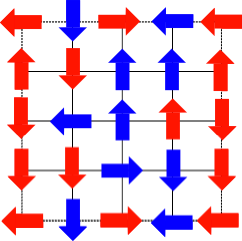
\includegraphics[scale=0.5]{PLG.png}\\
\textbf{Figure 1.} An example of a 2-D PLG model, with identity as color, orientation as arrow direction, and periodic boundary conditions applied.
\end{center}


\newpage


We will be using the Metropolis formulation of the Monte Carlo simulation in a canonical (constant-$NVT$) ensemble. A Metropolis Monte Carlo simulation has the following procedure:
\begin{itemize}
\item Pick a random move
\item Calculate the change in energy ($\Delta E$) associated with the random move
\item Calculate the Boltzmann probability $p = \min\left\{1, e^{-\Delta E/k_B T}\right\}$, where $k_B$ is the Boltzmann constant and $T$ is temperature
\item Calculate a random number $r \in [0,1]$
\item Accept the move if $p > r$, reject the move if $p \leq r$
\end{itemize}
\indent\indent In the canonical ensemble, the number of particles ($N$), volume ($V$), and temperature ($T$) are fixed. There are two types of allowed moves. The first is a rotation, where a random particle's orientation is changed. The second is a particle swap, where two particles in random locations are exchanged. The type of move is also chosen randomly, and the two moves have equal probability of occurring.\\
\indent The final simulation detail is the choice of Hamiltonian (i.e. how we calculate the energy of the system). For simplicity, we will use the following Hamiltonian:
$$H_0 = - \sum_{<i,j>}\delta_{m(i),m(j)} K + \delta_{s(i),s(j)} A$$
where $m(i)$ and $s(i)$ are the identity and orientation of particle $i$, and particles $i$ and $j$ are nearest neighbors. In plain English, if two neighboring particles have the same identity, they get a favorable energy bonus. Likewise, if two neighboring particles have the same orientation, they also get an energy bonus. This Hamiltonian is too simple to have any chemical application, but it makes a good test system for the efficiency of the algorithm.

\section*{Results \& Applications}
\vspace{-7pt}
\indent\indent This simulation is designed to study the mixing of two species and how they separate into different phases. We use two order parameters to determine different phases. The local composition parameter ($\theta$) and local orientation parameter ($\phi$) are defined below, where $M$ is the number of nearest neighbors included. For our purposes, we will use $M=26$, which corresponds to all the particles within a $3\times3\times3$ cube centered on particle $i$.
$$\theta(i) = \frac{1}{2} + \frac{1}{2M}\sum_j^M\delta_{m(i),m(j)}\left(\delta_{m(j),1}-\delta_{m(j),2}\right)$$
$$\phi(i) = \frac{1}{M}\sum_j^M\delta_{s(i),s(j)}$$
$\theta$ ranges from 0 (pure species 2) to 1 (pure species 1), with the intermediate value of 0.5 representing a perfect mixture. $\phi$ also ranges from 0 (total disorder) to 1 (perfect solid). A liquid phase would have an expected value of $\frac{1}{6}$ rather than 0 since particles should sometimes randomly match orientation.\\
\indent In order to smooth out the effect of defects, we calculate medium range order parameters, which are simply averages of the local order parameters. These parameters will allow use to calculate the compositions of separate phases and create phase diagrams.
$$\Theta(i) = \frac{1}{M}\sum_j^M\theta(j)$$
$$\Phi(i) = \frac{1}{M}\sum_j^M\phi(j)$$


\newpage


\section*{Proposed Parallelization Method}
\vspace{-7pt}
\indent\indent Semigrand canonical MC simulations have been successfully parallelized by a geometric division of the simulation. However, since the canonical ensemble includes particle swaps that can occur anywhere, a geometric division would require a large amount of communication. Instead, we propose that a scheme where one master thread generates moves and worker threads execute independent moves simultaneously. So long as the simulation size is much larger than the number of processors, the probability of conflicting moves being generated is fairly low.\\
\indent We are still discussing whether this program is better suited to MPI or shared memory. Both have their advantages and disadvantages. MPI would allow a huge number of processors to be added to the system, but ensuring that the system remains coherent could be problematic. Shared memory has no coherence issues so long as we avoid data races, but greatly limits the amount of processors that can be used. Regardless of which we decide to use, our proposed algorithm will do the following:
\begin{itemize}
\item Initialization of identity and orientation arrays
\item Processor 0 begins generating moves and keeping track of affected positions in an array
\item Proc 0 sends out moves to the remaining worker procs in a round robin fashion (resulting in a fairly balanced workload)
\item Move generation and execution will continue until a conflict is detected
\item In the simplest formulation, proc 0 will wait for all current moves to finish executing and reset the dirty positions array
\item Proc 0 will then restart move generation from the generated conflict until the next conflict
\item For data collection, proc 0 will ensure that all moves are complete to avoid read races
\item Data collection is a stencil computation and is easily parallelized by geometric division
\end{itemize}
\indent\indent A more sophisticated version of the algorithm could do several things to avoid the downtime due to synchronization during conflicts. Firstly, worker procs can notify the master thread when a move is complete, removing it from the dirty array and reducing the chance of having active conflicts. Secondly, a conflicting move can be safely assigned so long as it does not conflict with moves on two separate processors. This is because on each worker thread the program is being executed in serial, and therefore there is no possibility for a data race if the conflicting moves are assigned to the same thread.

\end{document}
